\documentclass{scrarticle}

\usepackage{circuitikz} %Für die Schaltpläne
\usepackage[T1]{fontenc} 
\usepackage[UTF8]{inputenc}
\usepackage{amsmath}
\usepackage{amssymb}
\usepackage{fancyhdr}
\usepackage{graphicx}
\usepackage{tikz}
\usepackage[ngerman]{babel}
    \usetikzlibrary{arrows,topaths}
\title{Elektrotechnik 1 - Praktikum 1}
\subtitle{Spannungs - und Stromquellen im belasteten Brückenschaltung}
\author{Karl Döring \and Florian Tietjen \and Eric Antosch}

\usepackage{amsthm}
\newtheorem{lemma}{Lemma}

\renewcommand\qedsymbol{$\square$}
\pagestyle{fancy}
\fancyhead[L]{\today}
\fancyhead[R]{ETP1}
\fancyfoot[L]{}
\fancyfoot[C]{\thepage}
\fancyfoot[R]{}
\begin{document}

\maketitle
\thispagestyle{empty}

\newpage

\tableofcontents
\thispagestyle{empty}

\newpage

\section{Vorwort}
Der Gegenstand unserer Untersuchungen entsprechen auf dem Papier nur der Änderung eines
Lastwiderstandes während einer bestimmten Zeit, und dessen Auswirkung auf der Rest der Schaltung (z.B. eine Brückenschaltung).
Wheatstonesche Brücken werden jedoch vermehrt in der Messtechnik eingesetzt, um bestimmte Werte messbar bzw. messbarer zu machen.

Dabei wird die Brücke über die anderen Widerstände abgeglichen, d.h. ein Messgerät, was an den Punkten A und B (siehe Abbildung unter 2.1)
angeschlossen werden würde, würde keine Potentialunterschiede und damit keine Spannung messen. Es kommt bei diesem Verfahren zu weniger Fehlern,
welche in manchen Geräten von sehr mächtiger Konsequenz sein können. Es ist daher ratsam, sich mit dem Einfluss von bestimmten Kenngrößen auf eine solche
Art von Schaltung eingehend Gedanken zu machen.

\section{Belastete Brückenschaltung an einer Spannungsquelle}

\begin{center}
  \begin{circuitikz}[european]
  \tikzstyle{obj}  = [circle, minimum width=5pt, fill, inner sep=0pt]
  \draw (0,0) to[V<=$U_0$, i_=$I_0$] (0,6) -- 
  (2,6) to[R, v=$U_1$, l=$R_1$, i^=$I_1$, *-] (2,4) -* (2,2)
  to[R=$R_2$, v=$U_2$, i^=$I_2$, *-*] (2,0) -- (0,0);
  \draw (2,6) -- (5,6) to[R=$R_3$, i^=$I_3$, v=$U_3$, -*] (5,4) -- (7,4)
   to[R=$R_L$, i_=$I_L$, fill=red!70!white] (7,2) -- (2,2);
  \draw (5,4) -- (5,2) to[R=$R_4$, v=$U_4$, i^=$I_4$] (5,0) -- (2,0);
  \draw[-latex] (6,3.5) -- (6,2.5);
  \draw (6,3) node[anchor=east] {$U_L$};
  \node [obj, label=above:A] (xa) at (6,4) {};
  \node [obj, label=below:B] (za) at (6,2) {};
\end{circuitikz}
\end{center}

\subsection{Vorbereitung}
\begin{abstract}
  \textbf{Aufgabe 1.1.1} Bestimmen Sie eine allgemeine Formel für die Berechnung der Ersatzspannungsquelle der Brückenschaltung,
  die in Abschnitt 2.1 angegeben ist, mit beliebigen $R_1, R_2, R_3, R_4$, wobei der Lastwiderstand $R_L$ nicht angeschlossen ist
  und geben Sie $U_q, I_k, R_i$ mit dieser Methode an.
\end{abstract}
Um hier auf die richtigen Lösung zu kommen, müssen wir die Potentiale $\phi_1$ und $\phi_2$ bestimmen, die an den Punkten A und B anliegen.
Hier können wir die Spannungsteilerregel anwenden, um auf den Wert $U_q$ zu kommen.
\begin{equation*}
  \begin{aligned}
    U_A &= U_0 \cdot \frac{R_3}{R_3+R_4}\\
    U_B &= U_0 \cdot \frac{R_1}{R_1+R_2}
  \end{aligned}
\end{equation*}
\begin{equation}\label{eq:Uq}
  U_q = U_{B-A} = U_0 \cdot \left(\frac{R_3}{R_3+R_4} - \frac{R_1}{R_1+R_2}\right)
\end{equation}
Für den Innenwiderstand der Ersatzspannungsquelle ergibt sich jetzt (siehe Anhang für das dafür genutzte Schaltbild):
\begin{equation}\label{eq:rg}
  \frac{1}{R_i} = \left(\frac{1}{R_1} + \frac{1}{R_2}\right) + \left(\frac{1}{R_3} + \frac{1}{R_4}\right)
\end{equation}
Durch die theoretischen Werte, die wir mit (\ref{eq:Uq}) und (\ref{eq:rg}) berechnet haben, können wir nun auch den fehlenden Wert $I_k$ berechnen:
\begin{equation}
  \label{eq:Ik}
  I_k = \frac{U_q}{R_i}
\end{equation}
\begin{abstract}
  \textbf{Aufgabe 1.1.2} Stellen Sie nun dar, was passieren würde, wenn alle $R_1 = R_3$ und $R_2 = R_4$
  gelten würde und was das für die Brückenschaltung bedeutet.
\end{abstract}
Da nun die oben genannten Bedingungen gelten, folgt, unabhängig von den Werten der Widerstände aus (\ref{eq:Uq}), dass 
die Quellenspannung der Ersatzspannungsquelle nun $0V$ beträgt. Demnach ist nun auch der Wert für $I_k = 0A$. Allein der Innenwiderstand der 
Ersatzspannungsquelle lautet nun:
\begin{equation*}
  \frac{1}{R_i} = \left(\frac{1}{R_1} + \frac{1}{R_2}\right) + \left(\frac{1}{R_3} + \frac{1}{R_4}\right) = 2\cdot\left(\frac{1}{R_1} + \frac{1}{R_2}\right)
\end{equation*}
\begin{abstract}
  \textbf{Aufgabe 1.1.3} Berechnen Sie nun den Wert der Quellenspannung $U_q$, des Innenwiderstands $R_i$ und des Kurzschlussstromes $I_k$ der Ersatzspannungsquelle.
\end{abstract}
Mit den oben gezeigten Formeln aus \textbf{Aufgabe 1.1.1} findet sich nun die Werte mit:
\begin{equation*}
  \begin{aligned}
    U_q &= U_{B-A} = U_0 \cdot \left(\frac{R_3}{R_3+R_4} - \frac{R_1}{R_1+R_2}\right) = 10V \cdot \left(\frac{10k\Omega}{10k\Omega+47k\Omega} - \frac{22k\Omega}{22k\Omega+33k\Omega}\right) = 2,2456V\\
    R_i &= \left(\frac{1}{R_i}\right)^{-1} = \left(\left(\frac{1}{R_1} + \frac{1}{R_2}\right) + \left(\frac{1}{R_3} + \frac{1}{R_4}\right)\right)^{-1} = \left(\left(\frac{1}{22k\Omega} + \frac{1}{33k\Omega}\right) + \left(\frac{1}{10k\Omega} + \frac{1}{47k\Omega}\right)\right)^{-1} = \\
    I_k &= \frac{U_q}{R_i} = \frac{2,2456V}{} = 
  \end{aligned}
\end{equation*}
\vspace{1.5cm}

\subsection{Simulation}


\subsubsection{Durchführung}
Wir simulieren nun in LTSpice mittels einer zeitabhängigen Funktion des $R_L$ (in der Grafik hellrot makiert) den Einfluss des Lastwiderstandes
auf die verschiedenen Werte der abgeglichnen belasteten Brückenschaltung und schauen uns zudem den Lastleistungswert an. 
Um diese Begebenheit in LTSpice zu simulieren, haben wir den Widerstandswert des Lastwiderstandes als Funktion der Zeit mit dem 
Proportionalitätsfaktor $2200$ erstellt und dann von $t_0 = 0s$ bis $t_{end} = 1000s$ die Wertänderung betrachtet. Die Werte werden dann über
sogenannte Traces von LTSpice auf dem Bildschirm ausgegeben. Diese werden dann als .txt-Tabelle exportiert und dann als Graph dargestellt (siehe Figure 1, siehe Anhang 1 für Tabelle).
\subsubsection{Beobachtung}
Die Werte für die Spannung ist in Rot in Abbildung 1 auf der nächsten Seite dargestellt. Man erkennt hier, dass, mit steigendem Widerstandswert,
auch die Spannung steigt. Jedoch ist der Verlauf nicht linear sondern nähert sich asymptotisch der Quellenspannung der Ersatzspannungsquelle
$U_q = 2,2456V$.
Typisch für die Kurve eines Leistungswerts am veränderlichen Lastwiderstand ist dieser an einem bestimmten Punkt am höchsten, sinkt danach aber wieder; wir bezeichnen
diesen Punkt im folgenden mit $P_{max}$.
\begin{figure}
  \begin{center}
    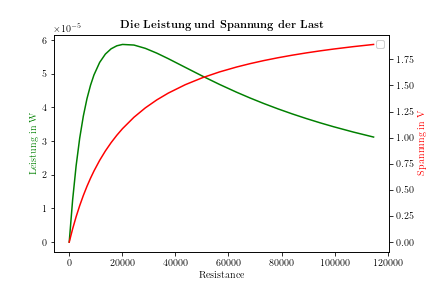
\includegraphics[scale=0.5]{pw_volt.png}
    \caption{Die Graphen der Leistung und Spannung in Abhängigkeit von dem Lastwiderstand $R_L$}
  \end{center}
\end{figure}
Der Punkt $P_{max}$ ist in diesem Fall der auf der Abbildung 1 erkennbare Hochpunkt der Funktion für die Lastleistung.
\begin{equation}\label{eq:pmax}
  \psi_n(\lambda, \mu) = \lambda \cdot \mu \land \lambda + \mu = x \in \mathbb{R} \text{ für beliebiges }n\in\mathbb{N}
\end{equation}
In der Aussage (\ref{eq:pmax}) definieren wir die Funktion der Leistung in Abhängigkeit von Strom und Spannung am Lastwiderstand. Wir überlegen uns, dass das Maximum der Leistung erreicht ist, wenn die Differenz der Stromstärke und der Spannung Null ist, sie also gleich sind. (Der Beweis findet sich im Anhang)
Grafisch lässt sich dieser Punkt als Schnittpunkt der Graphen für Strom und Spannung interpretieren (siehe Figure 2).
\begin{figure}
  \begin{center}
    \label{fig:all}
    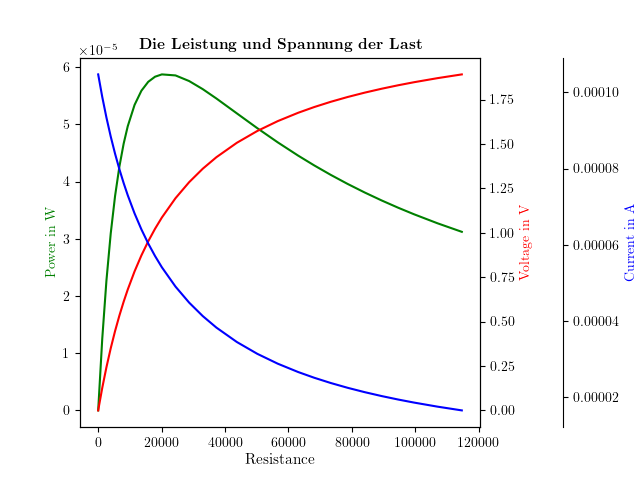
\includegraphics[scale=0.5]{pw_volt_rsv2.png}
    \caption{Die Graphen für die Spannung und den Strom treffen sich genau an dem Punkt, an welchem die Leistung maximal ist.}
  \end{center}
\end{figure}
Setzen wir nun alle anderen Werte als Funktion vom Widerstand, sondern betrachten den Wert der Stromstärke
als Funktion der Spannung, so bekommen wir eine wohlbekannte Generatorkennlinie, die ihren Nullpunkt auf dem Wert $U_q = 2,2456V$ und Y-Achsenabschnitt auf den Wert $I_k = $ hat und somit der Kennlinie unserer
Ersatzspannungsquelle entspricht (siehe Figure 3). Dieser Zusammenhang stellt wiederum nur erneut die Begebenheiten des Versuches dar,
da wir mit dem Kurzschlussstrom denjenigen Strom mit $\lim_{R_L\to 0} \frac{U_q}{R_G} = I_k$ und mit der Leerlaufspannung diejenige Spannung $\lim_{R_L\to\infty} I_k\cdot R_G = U_q$ bezeichnen, wobei im Falle der Ersatzspannungsquelle
$R_G = R_i + R_L$ gilt.
\begin{figure}
  \begin{center}
    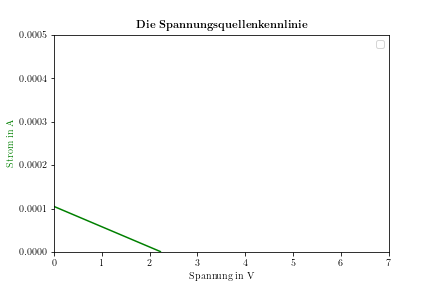
\includegraphics[scale=0.4]{curr_volt.png}
    \caption{Generatorkennlinie der Ersatzspannungsquelle}
  \end{center}
\end{figure}
\section{Belastete Brückengleichung an einer Stromquelle}
\begin{center}
  \begin{circuitikz}[european]
  \tikzstyle{obj}  = [circle, minimum width=5pt, fill, inner sep=0pt]
  \draw (0,0) to[isource, i_=$I_0$, l=$I_0$] (0,6) -- 
  (2,6) to[R, v=$U_1$, l=$R_1$, i^=$I_1$, *-] (2,4) -* (2,2)
  to[R=$R_2$, v=$U_2$, i^=$I_2$, *-*] (2,0) -- (0,0);
  \draw (2,6) -- (5,6) to[R=$R_3$, i^=$I_3$, v=$U_3$, -*] (5,4) -- (7,4)
   to[R=$R_L$, i_=$I_L$, fill=red!70!white] (7,2) -- (2,2);
  \draw (5,4) -- (5,2) to[R=$R_4$, v=$U_4$, i^=$I_4$] (5,0) -- (2,0);
  \draw[-latex] (6,3.5) -- (6,2.5);
  \draw (6,3) node[anchor=east] {$U_L$};
  \node [obj, label=above:A] (xa) at (6,4) {};
  \node [obj, label=below:B] (za) at (6,2) {};
\end{circuitikz}
\end{center}
\subsection{Vorbereitung}
\begin{abstract}
  \textbf{Aufgabe 1.2.1} Ermitteln Sie mithilfe der obenstehenden Zeichnung die Werte $R_i, U_q, I_k$ für die Ersatzspannungsquelle
  und geben Sie die allgemeinen Formeln für die Werte mit beliebigen $R_{1...4}$ an.
\end{abstract}
Um die Aufgabe so analog wie möglich zu gestalten, berechnen wir zuerst einmal den Gesamtwiderstand der vorliegenden Schaltung. Dieser wird berechnet durch:
\begin{equation}\label{eq:RG}
  \frac{1}{R_G} = \frac{1}{R_1 + R_2} + \frac{1}{R_3 + R_4}
\end{equation}
Zusammen mit dem Gesamtstrom $I_G$, der uns angegeben ist, können wir mit $R_G \cdot I_G = U_G$ berechnen. Ab hier können wir nun uns an der
\textbf{Aufgabe 1.1.1} orientieren und mit (\ref{eq:Uq}) den Wert $U_q$ erhalten. Nur der Innenwiderstand der Ersatzspannungsquelle unterscheidet sich noch
von dem vorherigen Wert, da die Stromquelle als Unterbrechung in der Leitung und nicht als Kurzschluss gewertet wird (siehe Anhang für entsprechende Zeichnung).
\begin{equation*}
  \frac{1}{R_i} = \frac{1}{R_1 + R_3} + \frac{1}{R_2 + R_4}
\end{equation*}
mit (\ref{eq:Ik}) können wir nun auch endlich den fehlenden Wert berechnen.
\begin{abstract}
  \textbf{Aufgabe 1.2.2} Berechnen Sie die Werte mithilfe der Formeln, die sie gerade erarbeitet haben und den vorgebenen Werten aus der Aufgabenstellung.
\end{abstract}
Wie in \textbf{Aufgabe 1.1.3} rechnen wir:
\begin{equation*}
  \begin{aligned}
    \left(\frac{1}{R_G}\right)^{-1} &= \left(\frac{1}{R_1 + R_2} + \frac{1}{R_3 + R_4}\right)^{-1} = \left(\frac{1}{55k\Omega} + \frac{1}{57k\Omega}\right)^{-1} = \\
    U_G &= I_G \cdot R_G = 1mA \cdot 5 = 5\\
  \end{aligned}
\end{equation*}
\subsection{Simulation}
\subsection{Durchführung}
Wir verwenden das gleiche Setup wie in der Durchführung des ersten Versuches, nur, dass wir hier eine Stromquelle verwenden.
Alle Werte werden wie gewohnt durch die Simulation errechnet und auf Graphen eingezeichnet.
\subsection{Beobachtung}
\begin{figure}
  \begin{center}
  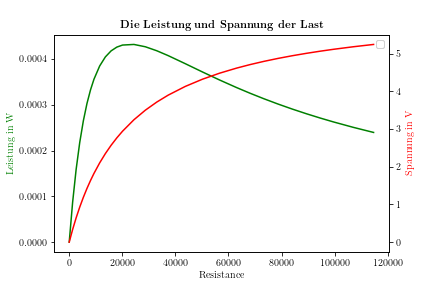
\includegraphics[scale=0.5]{pw_volt2.png}
  \caption{Die Leistung und Spannung des zweiten Versuches}
  \end{center}
\end{figure}
Auch hier ergibt sich ein ähnliches Schema, wie in Aufgabe 1. Sowohl Spannung als auch Strom nähern sich asymptotisch einem bestimmten Wert an ($\text{von }I_k\text{ für I, bis }U_q\text{ für U}$).
Analog zur gemachten Überlegung in (\ref{eq:pmax}) ist auch hier das Maximum der Leistungsfunktion bei dem Schnittpunkt der beiden Graphen zu sehen.
\begin{figure}
  \begin{center}
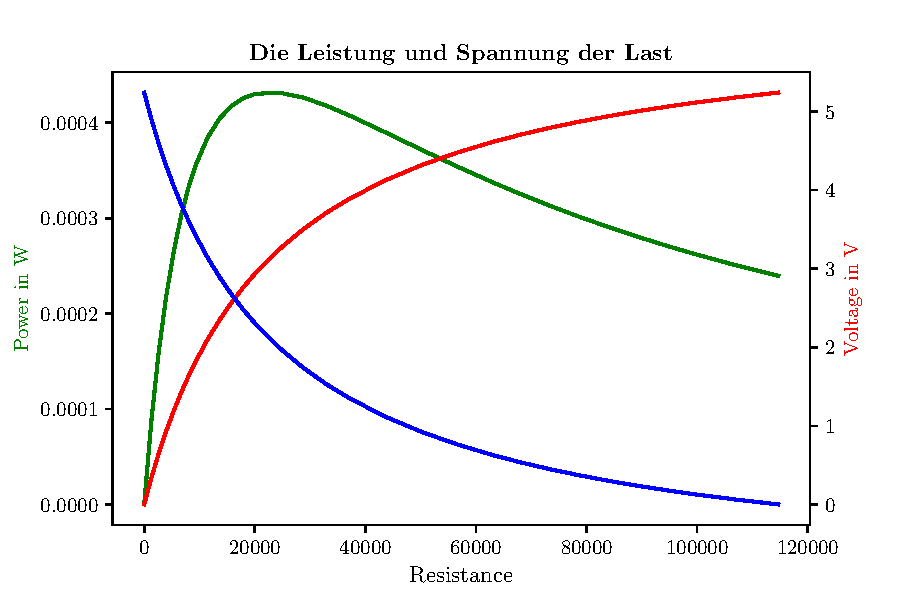
\includegraphics[scale=0.5]{pw_volt_rsjp2.pdf}
\caption{Der Schnittpunkt der beiden Were}
  \end{center}
\end{figure}

\section{Aufgabe 3}

\subsection{Vorbereitung}
\subsection{Simulation}

\section{Anhang}
\subsection{Beweis zu (\ref{eq:pmax})}
\begin{lemma}
  Sei $\psi\text{ eine Abbildung}, \lambda, \mu \in \mathbb{R}$, wobei $\psi_n(\lambda, \mu) = \lambda \cdot \mu \land \lambda + \mu = x \in \mathbb{R} \text{ für beliebiges }n\in\mathbb{N}$ ist. Es folgt, dass der Hochpunkt der Funktion an der Stelle ist, an der $\lambda - \mu = 0$ gilt.
\end{lemma}
\begin{proof}
  Wir wollen nun zunächst den Hochpunkt von $\psi_n$ berechnen. Dafür stellen wir $\lambda + \mu = x$ nach $\lambda$ um und erhalten $\lambda = x - \mu$.
  Im nächsten Schritt setzen wir die umgestellte Gleichung in unsere Funktion ein und erhalten $\psi(\mu) = \mu \cdot (x - \mu) = x\mu - \mu^2$. Um den Extrempunkt der Funktion zu erhalten, leiten wir zunächst die Funktion einmal ab:
  \begin{equation*}
    \psi'(\mu) = x-2\mu
  \end{equation*}
  Setzen wir die Funktion nun gleich Null, ergibt sich:
  \begin{equation*}
    \begin{aligned}
    0 &= x - 2\mu \\
    2\mu &= x \\
    \mu &= \frac{x}{2}
    \end{aligned}
  \end{equation*}
  Leiten wir nun die Funktion ein weiteres Mal ab und setzen unser $\mu$ von oben ein, erhalten wir:
  \begin{equation*}
    \psi''(\mu) = -2 < 0 \implies \mu\text{ ist Hochpunkt der Funktion}
  \end{equation*}
  Dadurch, dass dieser Vorgang analog mit $\lambda$ funktioniert, und das gleiche Ergebnis $\frac{x}{2}$ entsteht, ist das Lemma gezeigt.
\end{proof}
\subsection{Zeichnung zu der Widerstandsberechnung von 1 und 2}
\begin{center}
  

\begin{circuitikz}[european]
  \draw (0, 1) to[short, -*] (1,1) -- (1,2) to[R=$R_1$] (4,2) to[R=$R_3$] (7,2) to[short, -*] (7,1) -- (8,1);
  \draw (1,1) -- (1,0) to[R=$R_2$] (4,0) to[R=$R_4$] (7,0) to[short] (7,1);
  \draw[color=red] (4,2) to[short, *-*] (4,0);
  \node[anchor=south] (xa) at (0,1) {a};
  \node[anchor=south] (xb) at (8,1) {b};
\end{circuitikz}
\end{center}
Anmerkung: Für Aufgabe 1 ist die rote Verbindungslinie vorhanden, während bei Aufgabe 2 die Linie nicht mehr da ist.
\end{document}